\documentclass[notes]{subfiles}
\begin{document}
	\addcontentsline{toc}{section}{10.3 - Polar Coordinates}
	\refstepcounter{section}
	\fancyhead[RO,LE]{\bfseries \nameref{cs103}} 
	\fancyhead[LO,RE]{\bfseries \small \currentname}
	\fancyfoot[C]{{}}
	\fancyfoot[RO,LE]{\large \thepage}	%Footer on Right \thepage is pagenumber
	\fancyfoot[LO,RE]{\large Chapter 10.3}
	
\section*{Polar Coordinates}\label{cs103}
	\subsection*{Before Class}
	\subsection*{The Polar Coordinate System}
		\begin{question}
			The Cartesian coordinate system carries two pieces of information$-$ a horizontal distance, $x$, and a vertical distance, $y$.  If polar coordinates deal with circular objects, what two pieces of information should a polar coordinate carry?
		\end{question}
			\vspace{1.5in}
		\begin{ex}
			Use the polar grid below to plot the points.  Be sure to label your points.
		\end{ex}
			\begin{minipage}{1.5in}
				\begin{enumerate}[(a)]
					\setlength\itemsep{10pt}
					\item $\lrpar{2,-\dfrac{\pi}{6}}$
					\item $\lrpar{-3,\pi}$
					\item $\lrpar{1, \dfrac{\pi}{4}}$
					\item $\lrpar{4,-\dfrac{2\pi}{3}}$
					\item $\lrpar{-1,\dfrac{5\pi}{6}}$
					\item $\lrpar{2,0}$
				\end{enumerate}
			\end{minipage}
			\begin{minipage}{4.5in}
				\begin{center}
				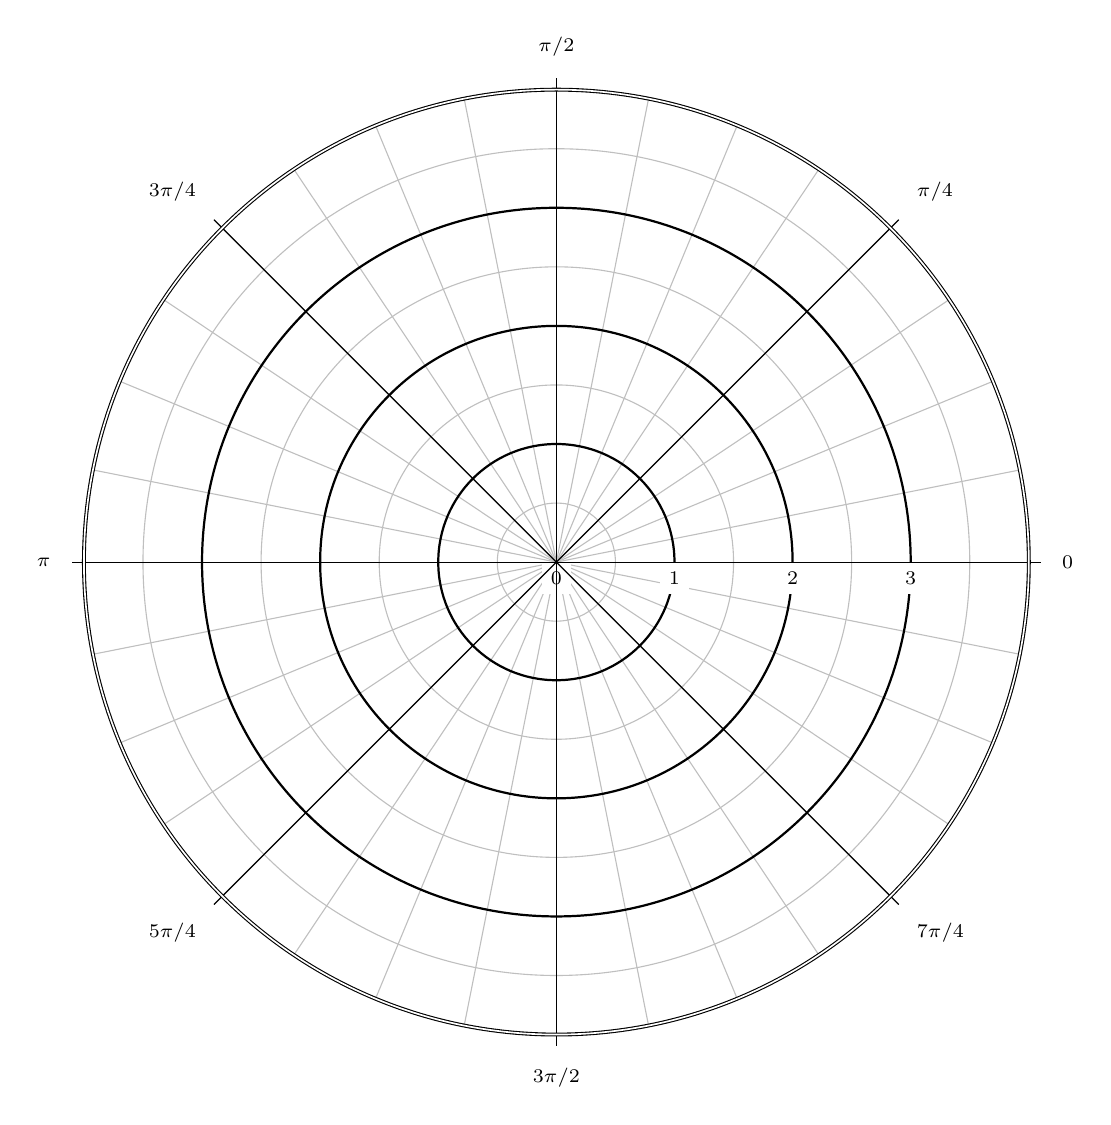
\begin{tikzpicture}[>=latex, scale = 1.5]
					% Draw the lines at multiples of pi/12
						\foreach \ang in {0,...,31} {
							\draw [lightgray] (0,0) -- (\ang * 180 / 16:4);
							}

					% Concentric circles and radius labels
						\foreach \s in {0, 1, 2, 3} {
							\draw [lightgray] (0,0) circle (\s + 0.5);
							\draw [thick](0,0) circle (\s);
							\node [fill=white] at (\s, 0) [below] {\scriptsize $\s$};
							}

					% Add the labels at multiples of pi/4
						\foreach \ang/\lab/\dir in {
  							0/0/right,
 							1/{\pi/4}/{above right},
 							2/{\pi/2}/above,
							3/{3\pi/4}/{above left},
							4/{\pi}/left,
							5/{5\pi/4}/{below left},
							7/{7\pi/4}/{below right},
							6/{3\pi/2}/below} {
								\draw (0,0) -- (\ang * 180 / 4:4.1);
								\node [fill=white] at (\ang * 180 / 4:4.2) [\dir] {\scriptsize $\lab$};
								}

					% The double-lined circle around the whole diagram
						\draw [style=double] (0,0) circle (4);

					\end{tikzpicture} 
					\end{center}
			\end{minipage}
				\newpage
				
		\begin{ex}
			Consider the polar point $\lrpar{1,\dfrac{\pi}{4}}$ plotted above.  This is not the \emph{only} way of describing the point.
				\begin{enumerate}[(a)]
					\item Give two or three different ways of expressing this point in polar coordinates.
						\vs{.5}
					\item Do you see a pattern in the expressions?  What is it?
						\vs{.5}
				\end{enumerate}
		\end{ex}
		
		\begin{rmk}[A Point in Polar Coordinates]
			Any point $(r,\theta)$ in polar coordinates can also be represented by the points\\[20pt] \blank{2.5} and \blank{2.5}.
		\end{rmk}
		
		There is a connection between Cartesian coordinates and polar coordinates; we can exploit trigonometry to find the relationship.\\[2pt]
			\begin{minipage}{3in}			
			\begin{ex}$ $
				\begin{enumerate}[(a)]
				\setlength\itemsep{10pt}
					\item At the right is a circle of radius $r$, with an inscribed right triangle.  Label as much as you can on the figure.
					\item Use the triangle and trigonometric functions to obtain a conversion from polar coordinates to Cartesian coordinates.
				\end{enumerate}				
			\end{ex}
			\end{minipage}
			\begin{minipage}{4in}
				\begin{center}
				\begin{tikzpicture}
					\draw (0,0) circle (4);
					\fill (0,0) circle (.1);
					\fill (2.81,2.81) circle (.1);
					\draw (0,0)--(2.81,2.81)--(2.81,0)--(0,0);
					\draw (2.81,0)--(2.81,.2)--(2.61,.2)--(2.61,0)--(2.81,0);
				\end{tikzpicture}
				\end{center}
			\end{minipage}
				\newpage
		
		\begin{rmk}[Polar-to-Cartesian Conversion]
			If a point $P$ has the polar coordinate expression $(r,\theta)$, then its Cartesian coordinate expression\\[20pt] is given by \blank{2} and \blank{2}. 
		\end{rmk}
		
		\begin{rmk}[Cartesian-to-Polar Conversion]
			If a point $P$ has the Cartesian coordinate expression $(x,y)$, then its polar coordinate expression\\[20pt] is given by \blank{2} and \blank{2}.
		\end{rmk}
		
		\begin{ex}
			Convert the following points from polar to Cartesian coordinates.
			\begin{enumerate}[(a)]
				\item $\lrpar{2,\dfrac{3\pi}{2}}$
					\vs{1}
				\item $\lrpar{\sqrt{2},\dfrac{\pi}{4}}$
					\vs{1}
				\item $\lrpar{-3,-\dfrac{\pi}{3}}$
					\vs{1}
			\end{enumerate}
		\end{ex}
		\begin{ex}
			Convert the following points from Cartesian to polar coordinates.
			\begin{enumerate}[(a)]
				\item $(-4,4)$
					\vs{1}
				\item $(\sqrt{3},1)$
					\vs{1}
				\item $(3,3\sqrt{3})$-
					\vs{1}
			\end{enumerate}
		\end{ex}
			\newpage
			
		\begin{ex}
			Convert each equation from polar to rectangular coordinates.  If possible, identify the curve.
			\begin{enumerate}[(a)]
				\item $r^2 = 16$
					\vs{1}
					
				\item $r = 4\sin\theta$
					\vs{1}
					
				\item $\theta =\dfrac{\pi}{3}$
					\vs{1}
					
				\item $r^2\cos2\theta = 1$
					\vs{1}
			\end{enumerate}
		\end{ex}
		
		\begin{ex}
			Convert each equation from rectangular coordinates to polar coordinates.
			\begin{enumerate}[(a)]
				\item $y = 2$
					\vs{1}
					
				\item $4y^2 = x$
					\vs{1}
					 
				\item $y = x$
					\vs{1} 
			\end{enumerate}
		\end{ex}
			\newpage
			
	\subsection*{Pre-Class Activities}
		\begin{ex}
			Use this space to write any questions you might have from the videos.
		\end{ex}
			\vs{1}
			
		\begin{ex}
			Plot each point below on a polar grid.  Then, convert each from polar coordinates to Cartesian coordinates.
			\begin{enumerate}[(a)]
				\item $\lrpar{2,\dfrac{5\pi}{6}}$
				\item $\lrpar{1,-\dfrac{2\pi}{3}}$
				\item $\lrpar{-1,\dfrac{5\pi}{4}}$
			\end{enumerate}
		\end{ex}
			\vs{1.5}
			
		\begin{ex}
			Convert $r = 4\csc\theta$ into rectangular coordinates, and describe/identify the graph.
		\end{ex}
			\vs{1}
			
		\begin{ex}
			Express the ellipse $\dfrac{x^2}{9} + \dfrac{y^2}{4} = 1$ in polar coordinates.
		\end{ex}
			\vs{1}
			\newpage
			
	\subsection*{In Class}
	\subsubsection*{Polar Curves}	
		\begin{ex}
			Graph the polar equation $\theta = \dfrac{\pi}{4}$
		\end{ex}
			\vs{1}
			
		\begin{ex}
			Let $r = 2\sin\theta$
			\begin{enumerate}[(a)]
				\item Make a table of values for the curve, for $0\leq\theta\leq\pi$
					\vs{2}
				\item Use the table to sketch the curve.
					\vs{1}
				\item Find the Cartesian equation for the curve.
					\vs{1}
			\end{enumerate}
		\end{ex}
			\newpage
			
		\begin{ex}
			Sketch the polar curve $r = 1 + \cos\theta$.  This shape is called a \emph{cardioid}.
		\end{ex}
			\vs{1}
			
		\begin{ex}
			Sketch the polar curve $r = \sin 2\theta$.  This shape is called a \emph{rose of four leaves}.
		\end{ex}
			\vs{1}
			\newpage
			
		\begin{rmk}[Symmetry in Polar Graphs]
			Consider the polar curve $r = f(\theta)$. 
			\begin{itemize}
				\setlength \itemsep{20pt}
				\item The curve is symmetric about the polar axis if \blank{2.5}.
				\item The curve is symmetric about the pole if \blank{2.8}.
				\item The curve is symmetric about $\theta = \dfrac{\pi}{2}$ if \blank{3}.
			\end{itemize}
		\end{rmk}
		
		\begin{ex}
			What kind of symmetries does the cardioid $r = 1 + \cos\theta$ possess?  What about the cardioid $r = 1+\sin\theta$?
		\end{ex}
			\vs{1}
			
		\begin{ex}
			Use symmetries to help you graph $r^2 = \cos 4\theta$.
		\end{ex}
			\vs{1}
			\newpage
			
	\subsubsection*{Tangents to Polar Curves}
		\begin{rmk}[Derivative of a Polar Curve]
			Given the polar curve $r = f(\theta)$, consider the parametric equations $x = $\blank{1.5}\\[20pt] and $y = $\blank{1.5}.  Then, \\ \\
				\[\dfrac{dy}{dx} = \hspace{3in}\]
		\end{rmk}
		\begin{pf}
		
		\end{pf}
			\vspace{1.5in}
			
		\begin{ex}
			Consider the cardioid $r = 1 + \sin\theta$.
				\begin{enumerate}[(a)]
					\item Find the slope of the tangent line when $\theta = \dfrac{\pi}{6}$.
						\vs{2}
					\item Find the points where the tangent line is horizontal or vertical.
						\vs{1}
				\end{enumerate}
		\end{ex}
			\newpage
			
		\begin{ex}
			Find the slope of the tangent line to the polar curve $r = 2\cos\theta$ at $\theta = \dfrac{\pi}{3}$.
		\end{ex}
			\vs{1}
			
		\begin{ex}
			Find the points on the curve $r = 1-\sin\theta$ where the tangent line is horizontal or vertical.
		\end{ex}
			\vs{1}
			\newpage
			
	\subsection*{After Class Activities}
		\begin{ex}
			Sketch the curve $r = 2(1+\cos\theta)$.  Then, convert the equation to Cartesian coordinates.
		\end{ex}
			\vs{1}
			
		\begin{ex}
			The graph below shows $r$ as a function of $\theta$, in Cartesian coordinates.  Use the graph to sketch the corresponding polar curve.\\
			\begin{flushleft}
				\includegraphics[scale = 1.25]{103_1.png}
			\end{flushleft}
		\end{ex}
			\vs{1}
			
		\begin{ex}
			Find the slope of the tangent line to the polar curve $r = 2 + \sin 3\theta$ at $\theta = \dfrac{\pi}{4}$.
		\end{ex}
			\vs{1}
			
\clearpage
\end{document}